\chapter{Machine learning challenges}
\label{cha:results}


\section{Text categorization}

When dealing with natural language, one of the most important common denominator is how we represent words as input to any of our models. How do we transform sentences/words into numerical vectors.

In this section, we will quickly describe Mikolov's Word2Vec models (Continuous Bag of Word, and Skip-Gram), that proposed a new way to build word embeddings based on words coocurrence in a context window.

Then we will explain in more detail recent work from Facebook, that proposes new models based on Mikolov's work, allowing the use of sub-word information, and proposing a novel way to compute classification tasks while learning embeddings.

\subsection{Probability of sequence of tokens}

One solution to extract information from a corpus of text is to build a model that will assign a probability to a sequence of tokens. 

Let's consider the following sentence: \say{\textit{To classify you have to learn.}}

A good language model will give this sentence a high probability because this is a completely valid sentence, syntactically and semantically.

Similarly, the sentence \say{Before car bird eating sea.} should have a very low probability because it makes no sense. 

Mathematically, we can call this probability on any given sequence of n words:

\begin{align}
	P(\textit{'To'},\textit{'classify'}, ..., \textit{'learn'})
\end{align}

To make sense, we would like sentences of a given corpus to have a high probability.

Let's introduce the notations for this section:

{\ttfamily
\begin{table}[H]
    \centering
    \begin{tabular}{ll}
        \toprule
        $V$       	   	 &    the ordered vocabulary \\
        $T$    		   	 &    the size of corpus \\
        $w_i$          	 &    the i-th word in corpus \\
        $v_{i}$          	 &    the i-th word in vocabulary \\
        $V(w_i)$       &    the index of i-th word of corpus in vocabulary V, such as $ w_{i} = v_{V(w_i)}$\\
        $C_t^{(c)}$      &    the context of t-th word in corpus, for window of size $c$: $w_{t-c}, ..., w_{t-1}, w_{t+1}, ... ,w_{t+c}$\\
		$\mathbf{x}_i$ 				& one hot word vector corresponding i-th word in vocabulary $V$ \\
        $\mathbf{\bar x_t}$ 	& the average of all one hot vectors of words in context $C_t^{(c)}$ \\
        \bottomrule
    \end{tabular}
\end{table}
}

With:
\begin{align}
	\mathbf{x}_1 &= 
	\begin{bmatrix} 
		1 \\
		0 \\
		\vdots\\
		0
	\end{bmatrix} \\
	\mathbf{\bar x_t} &= \frac{\mathbf{x}_{V(t-c)} + \mathbf{x}_{V(t-c+1)} ... + \mathbf{x}_{V(t+c)}}{|C_t^{(c)}|}
\end{align}

Taking our corpus \say{\textit{To classify you have to learn.}}:

\begin{itemize}
	\item our corpus is of size: $T=6$
	\item our vocabulary is: $V =$ (to, classify, you, have, learn), an ordered list of size $|V| = 5$ (word \textbf{to} is present twice in corpus)
	\item $w_5$ is word \textbf{to}, indexed in vocabulary as $V(w_5) = 1$ (first word of vocabulary), ie $w_5 = v_1$
	\item $\mathbf{x}_{V(w_5)} = \mathbf{x}_{1} = \begin{bmatrix} 
		1 \\
		0 \\
		\vdots\\
		0
	\end{bmatrix}$
	\item $C_3^{(2)}$ is context of word \textbf{you} with window of size 2: \{to, classify, have, to\}
	\item 
		\begin{align}
		\mathbf{\bar x_t} &= (\mathbf{x}_{V(w_1)} +\mathbf{x}_{V(w_2)} + \mathbf{x}_{V(w_4)} + \mathbf{x}_{V(w_5)}) / 4 \\ 
		&= (\mathbf{x}_{1} +\mathbf{x}_{2} + \mathbf{x}_{4} + \mathbf{x}_{1}) / 4 
		=\begin{bmatrix} 
			1/2 \\
			1/4 \\
			0\\
			1/4\\
			0
		\end{bmatrix}
	\end{align}
\end{itemize}


\subsection{Word2Vec models}

Word2vec consists in either of two model architectures to produce a representation of words: \textbf{continuous bag-of-words} (CBOW) or \textbf{skip-gram}. 

In the continuous bag-of-words architecture, the model predicts the current word from a window of surrounding context words. The order of context words does not influence prediction (bag-of-words assumption). In the continuous skip-gram architecture, the model uses the current word to predict the surrounding window of context words. 
The skip-gram architecture weighs nearby context words more heavily than more distant context words.

Both models can be trained from an unlabeled large corpus of text and rely on the same trick: transform unlabeled data into a labeled dataset for supervised learning to unveil hidden dependencies between words.

Since these two models are quite similar, we will only describe in detail the CBOW in this section.

\subsubsection{CBOW}

In the CBOW model, we try to maximize the likelihood occurence of a word given its context, for a given window size.

Taking our previous corpus: \say{\textit{To classify you have to learn.}}


With a context window of size 2, we can extract many labeled samples:
\begin{itemize}
	\item \textbf{context}: \{classify, you\}, \textbf{target}: to
	\item \textbf{context}: \{to, you, have\}, \textbf{target}: classify
	\item \textbf{context}: \{to, classify, have, to\}, \textbf{target}: you
	\item ...
	\item \textbf{context}: \{have, to\}, \textbf{target}: learn
\end{itemize}


Mathematically, with $w_t$ our target word, $c$ the size of our context window, the probability of our target word given the context can be written as:

\begin{align}
	P(w_t | w_{t-c}, ..., w_{t-1}, w_{t+1}, ... ,w_{t+c}) = P(w_t | C_t^{(c)})
\end{align}

Given a word vocabulary of size $V$, the goal is to learn a vectorial representation for each word $w$. Word representations are trained to \emph{predict well} words that appear in its context.

So given a large training corpus represented as a sequence of words $w_1, ..., w_T$, the objective of the CBOW model is to maximize the following log-likelihood:
\begin{equation*}
  \sum_{t=1}^T \ \log P(w_t \ | \ \mathcal{C}_t^{(c)}),
\end{equation*}

\textbf{Parametrization and model}

The probability of observing a context word $w_t$ given $\mathcal{C}_t^{(c)}$ will be parameterized using the aforementioned word vectors.

We create two matrices $A \in \mathbb{R}^{dim \times |V|}$ and $B \in \mathbb{R}^{|V| \times dim}$, where $dim$ is an arbitrary size which defines the size of our embedding space.

$A$ is the input word matrix such that the i-th column of $A$ is the embedded vector of dimension \textit{dim} for word $v_{i}$ when it is an input to this model. 
Similarly, B is the output word matrix. The j-th row of B is an embedded vector of dimension \textit{dim} for word $v_j$ when it is an output of the model. 


Let's introduce some new notations:

{\ttfamily
\begin{table}[H]
    \centering
    \begin{tabular}{ll}
        \toprule
        $dim$ 				& chosen size for our embeddings \\
        $A$ 				& input word matrix $\in \mathbb{R}^{dim \times |V|}$ \\
        $B$ 				& output word matrix $\in \mathbb{R}^{|V| \times dim}$ \\
        \bottomrule
    \end{tabular}
\end{table}
}

The input matrix A converts our encoded input bag of words ($\mathbf{\bar x_t} $) into a representation in a lower dimensionality.

Let's denote our hidden representation:
\begin{align}
 \mathbf{h}_t = A.\mathbf{\bar x_t}
\end{align}

Finally, this hidden representation will be decoded with the output matrix B to be able to compare it with our target word. Since we are in a single labeled multiclass case, the use of softmax function is adapted to sum our probabilities to 1. In short, in CBOW we define the probability of occurence of each word of the vocabulary, given a context $\mathcal{C}_t^{(c)}$ (our model), as:

\begin{align}
 \mathbf{\hat y}_t = 
	\begin{bmatrix} 
		P(v_1 | \mathcal{C}_t^{(c)}) \\
		\vdots \\
		P(v_t | \mathcal{C}_t^{(c)})\\
		\vdots \\
		P(v_{|V|} | \mathcal{C}_t^{(c)})
	\end{bmatrix} = 
	softmax(B.A.\mathbf{\bar x_t} )
\end{align}

Ie $\forall i \in [1, |V|]$:
\begin{align}
 P(v_i | \mathcal{C}_t^{(c)})= 
 	&\frac{  [e^{B.A.\mathbf{\bar x_t}}]_i}
 	{\sum_{j=1}^{|V|} [e^{B.A.\mathbf{\bar x_t}} ]_j} \\
 	\text{      with}& []_i \text{ meaning the i-th element of a vector}
\end{align}


Whereas the true target is noted (target word in vocabulary):
\begin{align}
 \mathbf{y}_t = 
	\begin{bmatrix} 
		0 \\
		\vdots \\
		1 \\
		\vdots \\
		0
	\end{bmatrix} 
	= \mathbf{x}_{V(w_t)}
\end{align}


Since $\mathbf{y}_t$ is a one-hot vector (with 1 at location $V(w_t)$), maximizing log-likelihood of $P(w_t | \mathcal{C}_t^{(c)})$ is equivalent to minimizing the cross entropy of $(\mathbf{\hat y}_t, \mathbf{y}_t)$:
\begin{align}
E(\mathbf{\hat y}_t, \mathbf{y}_t) &= - \mathbf{y}_t^{\top} log(\mathbf{\hat y}_t) = - log(P(v_{V(w_t)} | \mathcal{C}_t^{(c)})) =- log(P(w_t | \mathcal{C}_t^{(c)}))
\end{align}

We can represent it as the following multilayer network:

\begin{tikzpicture}[shorten >=1pt,->,draw=black!50, node distance=\layersep]
    \tikzstyle{every pin edge}=[<-,shorten <=1pt]
    \tikzstyle{neuron}=[circle,fill=black!25,minimum size=17pt,inner sep=0pt]
    \tikzstyle{input neuron}=[neuron, fill=yellow!50];
    \tikzstyle{output neuron}=[neuron, fill=blue!50];
    \tikzstyle{hidden neuron}=[neuron, fill=red!50];
    \tikzstyle{true neuron}=[neuron, fill=green!50];
    \tikzstyle{annot} = [text width=4em, text centered]

    % Draw the input layer nodes
    \foreach \name / \y / \word in {1/1/to,2/2/classify,3/3/you,4/4/have,5/5/learn}
        \node[input neuron, pin=left: (\textit{\word}) $x_{\y}$ ] (I-\name) at (0,-0.5 -\y) {};

    % Draw the hidden layer nodes
    \foreach \name / \y in {1,...,3}
        \node[hidden neuron] (H-\name) at (\layersep,-1 -\y) {};
    
    % Draw the output layer node

	\foreach \name / \y in {1,...,5}
        \node[output neuron, pin=right:$\hat y_{\y}$ ] (O-\name) at (\layersep*2,-0.5 -\y) {};

    % Draw the true layer node
	\foreach \name / \y / \word in {1/1/to,2/2/classify,3/3/you,4/4/have,5/5/learn}
        \node[true neuron, pin=right:$y_{\y} (\textit{  \word})$ ] (T-\name) at (\layersep*3,-0.5 -\y) {};


    % Connect every node in the input layer with every node in the
    % hidden layer.
    \foreach \source in {1,...,5}
        \foreach \dest in {1,...,3}
            \path (I-\source) edge (H-\dest);

    % Connect every node in the hidden layer with the output layer
    \foreach \source in {1,...,3}
        \foreach \dest in {1,...,5}
	        \path (H-\source) edge (O-\dest);

    % Annotate the layers
    \node[annot,above of=H-1, node distance=2.5cm] (hl) {Hidden layer: $\mathbf{h}$ of size \textit{dim}};
    \node[annot,left of=hl] {Input layer: $\mathbf{x}$ (size $|V|$)};
    \node[annot,right of=hl] (ol) {Output layer: $\mathbf{\hat y}$ of size $|V|$};
    \node[annot,right of=ol] {Target: $\mathbf{y}$ one hot vector of size $|V|$};

    \node[annot] (A) at (\layersep/2,-5) {$A$};
    \node[annot] (B) at (\layersep*3/2,-5) {$B$};

\end{tikzpicture}

Matrices A and B are updated using gradient descent and gradient retro-propagation.

\subsubsection{Using CBOW embeddings for classification}

Using CBOW algorithm would provide you this A matrix, which is basically a lookup table in which you can extract the representation of any word of your vocabulary in your embedding space (of size $dim <<< |V|$).

Word2Vec treats each word in corpus like an atomic entity and generates a vector for each word.

Transforming a text input in a numerical vector is then possible, and your numerical vector could then be used as input for any classification algorigthm to perform classification tasks.

\subsection{Fasttext}

Fasttext, which is essentially an extension of word2vec model, brings two major conceptual changes (in addition to a very efficient C++ implementation):
\begin{itemize}
	\item simulatenous embedding and classification learning: in Word2Vec, we first build our embeddings, and then use it to translate words in features of low dimensionality for further classification. In fasttext, embedding and classification are different layers of a neural network that are trained simultaneously.
	\item use of subword word information, instead of treating only word entities
\end{itemize}

Details can be found in two papers published by Fasttext team: \cite[Enriching Word Vectors with Subword Information]{fasttextEnriching} and \cite[Bag of Tricks for Efficient Text Classification]{fasttextTricks}

\subsubsection{Multiclass classification model}

Let's consider the case where we have a training set of multiclass single-labeled sentences, for instance:
\begin{itemize}
	\item \textbf{feature}: \{I'm hungry\}, \textbf{target}: neutral 
	\item \textbf{feature}: \{Get out\}, \textbf{target}: angry
	\item \textbf{feature}: \{Nice to be there\}, \textbf{target}: happy
	\item ...
	\item \textbf{feature}: \{Do you want this apple\}, \textbf{target}: curious
\end{itemize}
With our target space being: \{happy, angry, neutral, curious\}, of size $K=4$

What fasttext does, is that instead of first learning word embeddings on a corpus of text, it directly uses features to build specialized embeddings for this classification task.

Denoting $\mathcal{Y} = \{y_i\}_{i \in [1, K]}$, and $\mathbf{x}$ the average of one hot-encoded vector of tokens of a feature in vocabulary $V$:
\begin{align}
 \mathbf{\hat y} 
 = 
	\begin{bmatrix} 
		\hat y_1 \\
		\vdots \\
		\hat y_i\\
		\vdots \\
		\hat y_K
	\end{bmatrix} 
 =	\begin{bmatrix} 
		P(y_1 | \mathbf{x}) \\
		\vdots \\
		P(y_i | \mathbf{x})\\
		\vdots \\
		P(y_K | \mathbf{x})
	\end{bmatrix} = 
	softmax(B.A.\mathbf{x})
\end{align}

Ie $\forall i \in [1, K]$:
\begin{align}
 P(y_i | \mathbf{x})= 
 	&\frac{  [e^{B.A.\mathbf{x}}]_i}
 	{\sum_{j=1}^{K} [e^{B.A.\mathbf{x}}]_j} \\
 	\text{      with}& []_i \text{ meaning the i-th element of a vector}
\end{align}


Whereas the true target is noted:
\begin{align}
 \mathbf{y} = 
	\begin{bmatrix} 
		y_1 \\
		\vdots \\
		y_i \\
		\vdots \\
		y_K
	\end{bmatrix} 
\end{align}
wich is a one hot encoded vector corresponding to which is this sample label.


The model is very similar to continuous bag of words model, except that instead of using the middle word of CBOW, we directly use a label. The architecture is then:
\begin{tikzpicture}[shorten >=1pt,->,draw=black!50, node distance=\layersep]
    \tikzstyle{every pin edge}=[<-,shorten <=1pt]
    \tikzstyle{neuron}=[circle,fill=black!25,minimum size=17pt,inner sep=0pt]
    \tikzstyle{input neuron}=[neuron, fill=yellow!50];
    \tikzstyle{output neuron}=[neuron, fill=blue!50];
    \tikzstyle{hidden neuron}=[neuron, fill=red!50];
    \tikzstyle{true neuron}=[neuron, fill=green!50];
    \tikzstyle{annot} = [text width=4em, text centered]

    % Draw the input layer nodes
    \foreach \name / \y / \word in {1/1/I,2/2/am,3/3/hungry,4/4/get,5/5/out, 6/6/nice, 7/7/apple}
        \node[input neuron, pin=left:(\textit{\word  }) $x_{\y}$ ] (I-\name) at (0,-\y) {};

    % Draw the hidden layer nodes
    \foreach \name / \y in {1,...,3}
        \node[hidden neuron] (H-\name) at (\layersep,-1 -\y) {};

    % Draw the output layer node
	\foreach \name / \y in {1,...,4}
        \node[output neuron, pin=right:$\hat y_{\y}$ ] (O-\name) at (\layersep*2,-0.5 -\y) {};

    % Draw the true layer node
	\foreach \name / \y / \label in {1/1/happy,2/2/neutral, 3/3/curious,4/4/angry}
        \node[true neuron, pin=right:$y_{\y}$ (\textit{  \label})] (T-\name) at (\layersep*3,-0.5 -\y) {};

    % Connect every node in the input layer with every node in the hidden layer.
    \foreach \source in {1,...,7}
        \foreach \dest in {1,...,3}
            \path (I-\source) edge (H-\dest);

    % Connect every node in the hidden layer with the output layer
    \foreach \source in {1,...,3}
        \foreach \dest in {1,...,4}
	        \path (H-\source) edge (O-\dest);

    % Annotate the layers
    \node[annot,above of=H-1, node distance=2.5cm] (hl) {Hidden layer: $\mathbf{h}$ of size \textit{dim}};
    \node[annot,left of=hl] {Input layer: $\mathbf{x}$ (size $|V|$)};
    \node[annot,right of=hl] (ol) {Output layer: $\mathbf{\hat y}$ of size $K$};
    \node[annot,right of=ol] {Target: one hot vector $\mathbf{y}$ of size $K$};

    \node[annot] (A) at (\layersep/2,-6) {$A$};
    \node[annot] (B) at (\layersep*3/2,-5) {$B$};

\end{tikzpicture}
Note: 
\begin{itemize}
	\item for readibility just 7 words of the input features are considered.
	\item fasttext first merge all features as one corpus to build vocabulary ($\rightarrow$ size of matrix A)
	\item in practice, dimension of the hidden layer is between 50 and 300
	\item input matrix A embeddings are specialized for this classification task and may not behave well for another classification task
	\item the target vector is exactly composed of one 1, and the rest of 0s (multi-class).
\end{itemize}

\textbf{Subword information}

Each word can be considered as a set of character ngrams. In Fasttext, a word vector is made of the sum of this character n grams. For example the word vector “apple” is a sum of the vectors of the n-grams:
\begin{multicols}{4}
\begin{itemize}
	\item “<ap”, 
	\item “app”, 
	\item ”appl”, 
	\item ”apple”, 
	\item ”apple>”, 
	\item “ppl”, 
	\item “pple”, 
	\item ”pple>”, 
	\item “ple”, 
	\item ”ple>”, 
	\item ”le>”
\end{itemize}
\end{multicols}
Note: this behavious is controlled through hyperparameters controlling smallest ngram size ([minn]) and largest ngram size ([maxn]). For performance and memory size reasons, another hyperparameter ([bucket]) controls the maximum total number of tokens (word tokens + subword tokens).

This provide the following advantages:
\begin{itemize}
	\item Generate better word embeddings for rare words (even if words are rare their character n grams are still shared with other words - hence the embeddings can still be good). In word2vec a rare word (e.g. 10 occurrences) has fewer neighbors to be tugged by, in comparison to a word that occurs 100 times - the latter has more neighbor context words and hence is tugged more often resulting in better word vectors.
	\item Out of vocabulary words - they can construct the vector for a word from its character n grams even if word doesn't appear in training corpus. The choice of hyper parameters controlling the minimum and maximum n-gram sizes has to be chosen.
\end{itemize}

Concretely, the use of subword information will only impact:
\begin{itemize}
	\item how is built the vocabulary. It will not only contain words of the training corpus, but also all ngrams of these words. The vocabulary will thus be much bigger, but with shared properties between different words.
	\item how features are encoded in this vocabulary: 'Do you want this apple' will not be encoded as the average of 5 one hot vectors \{do, you, want, this, apple\}, but as the average of one hot vectors of all tokens contained in the sentence \{<do>, <you, you>, <wa, wan, ant, nt> ...\}.
\end{itemize}

\subsubsection{Optimization}

Fasttext comes with some optimizations to compute efficent softmax approximations: hierarchical softmax and negative sampling. These techniques are detailed in \cite{fasttextTricks}.

\pagebreak
\section{Multilabel classification}

We already studied in previous section how we could compute efficient multi-class classification from natural language input. Yet in our project, most of the product attributes that we wanted to predict were multi-labeled.

In this section, we will first make a quick review of the major algorithms and scoring metrics for multi-label classification, mainly based on the ~\cite[following paper]{MultilabelReview}. Then we will focus on another common approach in neural networks not detailed in the previous paper, that inspired us to modify fasttext algorithm to make it natively support multilabel classification.


\subsection{Multilabel metrics}

Suppose $\mathcal{X} = \mathbb{R}^d$ denotes the \textit{d}-dimensional instance space, and  $\mathcal{Y} = \{y_1, y_2, \dots, y_K \}$ the label space with $K$ possible class labels.

Let's denote $\mathcal{D} = \{(\mathbf{x}_i, Y_i) | 1 \leq i \leq n\}$ our learning dataset. For each multi-label example $(\mathbf{x}_i, Y_i)$, $Y_i \subseteq \mathcal{Y}$ is the set of labels for $\mathbf{x}_i$.

\subsubsection{Common dataset description metrics}

\begin{itemize}
	\item \textbf{Number of classes}: $|\mathcal{Y}| = K$.
	\item \textbf{Label cardinality}: $\frac{1}{n}\sum_{i=1}^n |Y_i|$ (average number of labels per sample).
	\item \textbf{Label density}: $\frac{1}{n \times |\mathcal{Y}|}\sum_{i=1}^n |Y_i|$ (average number of labels per example normalized by number of classes).
	\item \textbf{Label diversity}: $|\{Y | \exists \mathbf{x}:(\mathbf{x}, Y) \in \mathcal{D}\}|$ (the number of distinct label sets in learning set).
\end{itemize}


\subsubsection{Scoring metrics}

In multi-label context, scoring metrics can be divided in two groups \cite{MultilabelReview}: 
\begin{itemize}
	\item sample-wise metrics: how well we performed on a sample
	\item label-wise metrics: how well we performed on a given class
\end{itemize}

In our case, the metrics of most interest are label-wise metrics, we will detail those we consider, which are derived from binary classification scoring metrics.  

Denoting $f$ our classifier, let's define the following metrics, for each class independently:
$\forall j \in [1, K]$:
{\ttfamily
\begin{table}[H]
    \centering
    \begin{tabular}{ll}
        \toprule
        $TP_j = |\{ \mathbf{x}_i | y_j \in Y_i \wedge y_j \in f(\mathbf{x}_i), 1 \leq i \leq n \}|$          &    $true\ positives\ for\ class\ j$ \\
        $FP_j = |\{ \mathbf{x}_i | y_j \notin Y_i \wedge y_j \in f(\mathbf{x}_i), 1 \leq i \leq n \}|$          &    $false\ positives\ for\ class\ j$ \\
        $TN_j = |\{ \mathbf{x}_i | y_j \notin Y_i \wedge y_j \notin f(\mathbf{x}_i), 1 \leq i \leq n \}|$       &    $true\ negatives\ for\ class\ j$  \\
        $FN_j = |\{ \mathbf{x}_i | y_j \in Y_i \wedge y_j \notin f(\mathbf{x}_i), 1 \leq i \leq n \}|$       &    $false\ negatives\ for\ class\ j$  \\
        \bottomrule
    \end{tabular}
\end{table}
}

Let $B(TP_j, FP_j, TN_j, FN_j)$ represent some binary classification metric among those of most interest for us: Precision, Recall, $F_{\beta}$ score (detailed in appendix). 

These metrics can be considered as \textit{local} metrics: each is specific to a given class. To obtain what we can could call \textit{global} metrics, that represent performance on all classes, two kinds of averaging can be considered:

\begin{itemize}
	\item Macro-averaging: equal weights for labels.
	\begin{align}
		B_{macro}(h) = \frac{1}{K}\sum_{j=1}^K B(TP_j, FP_j, TN_j, FN_j)
	\end{align}
	\item Micro-averaging: equal weights for samples.
	\begin{align}
		B_{micro}(h) = B(\sum_{j=1}^K TP_j, \sum_{j=1}^K FP_j,\sum_{j=1}^K  TN_j,\sum_{j=1}^K  FN_j)
	\end{align}
\end{itemize}


Those two averaging answer to different challenges. A high micro-averaged score can hide very poor results on classes with few occurences. A high macro-averaged score will give the same impact for a class with 1000 samples and another class of 2 samples. Both have their benefits and weaknesses depending on your goal.

In our case, our interest was more focused on micro-averaging, and classes with too poor local metrics are filtered after prediction.

\subsection{Output size challenge}

The key challenge of learning from multi-label data lies in the overwhelming size of output space, i.e. the number of label sets grows exponentially as the number of class labels increases. For example, for a label space with 20 class labels, the number of possible label sets would exceed one million ($2^{20}$).

Existing strategies to label correlations exploitation can be categorized based on the order of correlations that the learning techniques have considered:
\begin{itemize}
	\item First-order strategy: The task of multi-label learning is tackled in a label-by-label style and thus ignoring co-existence of the other labels, such as decomposing the multi-label learning problem into a number of independent binary classification problems (one per label). 
	\item Second-order strategy: The task of multi-label learning is tackled by considering pairwise relations between labels, such as the ranking between relevant label and irrelevant label , or interaction between any pair of labels, etc.
	\item High-order strategy: The task of multi-label learning is tackled by considering high-order relations among labels such as imposing all other labels’ influences on each label, or addressing connections among random subsets of labels, etc.
\end{itemize}

There is a compromise to find between taking into account correlations between labels, or choosing computational efficiency: the computational complexity quickly increase.

\subsection{Multi-label learning algorithms}

Multilabel strategies can be grouped in two main approaches: problem transformation methods or algorithm adaptation methods.

Briefly, the key philosophy of problem transformation methods is to fit data to algorithm,
while the key philosophy of algorithm adaptation methods is to fit algorithm to data. Figure ~\ref{fig:multilabelOverview}
summarizes the algorithms detailed in \cite[Zhang and Zhou paper]{MultilabelReview}.

\textbf{Algorithm adaptation methods}

This category of algorithms tackle multi-label learning problem by adapting popular learning techniques to deal with multi-label data directly. Each technique is thus specific to one algorighm.
Some adaptative algorithm exist for lazy learning techniques (kNN), decision tree techniques, kernel techniques (SVM), information-theoretic techniques (CRF).

\textbf{Problem transformation methods}

This category of algorithms tackle multi-label learning problem by transforming it into other well-established learning scenarios (binary or multiclass classification scenarios). 
Representative algorithms include:
\begin{itemize}
 \item Binary Relevance: which transform the task of multi-label learning into the task of binary classification (first-order)
 \item Classifier Chains: which transform the task of multi-label learning into the task of binary classification (high-order)
 \item Calibrated Label Ranking: which transforms the task of multi-label learning into the task of label ranking (second-order)
 \item Random k-labelsets which transforms the task of multi-label learning into the task of multi-class classification (high-order)
\end{itemize}

\begin{figure}[H]
\centering
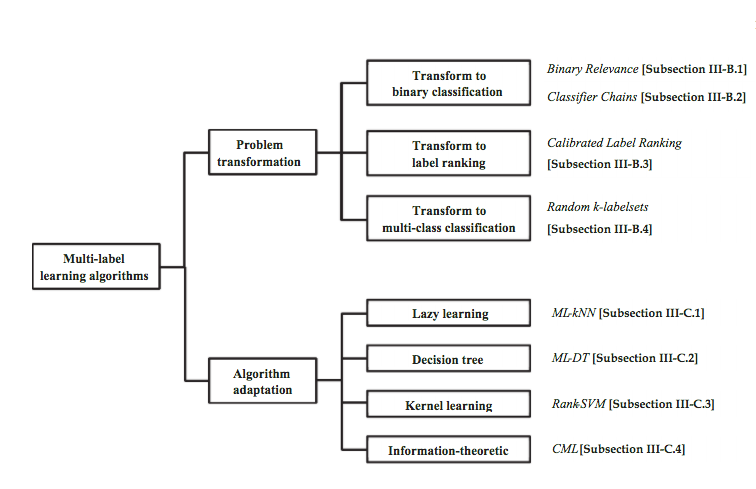
\includegraphics[scale=0.6]{./images/machine-learning/multi-label-approaches.png}
\caption{Categorization of representative multi-label learning algorithms reviewed in \cite[this paper]{MultilabelReview}.}
\label{fig:multilabelOverview}
\end{figure}


\subsection{Considered approaches}

In our case, the possible approaches were:
\begin{itemize}
	\item 'Word Embedding / Multi-label Classification':
	\begin{itemize}
		\item first learn general purpose word embeddings
		\item and then apply any multi-label classifier strategy
	\end{itemize}
	\item 'Fasttext / Problem Transform approach'
	\begin{itemize}
		\item use fasttext as binary/multiclass classifier
		\item as input for a problem transform approach: binary relevance, random-k-labelsets (classifier chains was not adaptable to fasttext)
	\end{itemize}
	\item adapt fasttext to support multi-label: learn simultanously embeddings and classifier parameters in multilabel context
\end{itemize}

\subsubsection{Project constraints}

Among our objectives were:
\begin{itemize}
	\item minimize the complexity of the workflow
	\item minimize number of different languages in the whole pipeline (previously spark)
	\item run fitting on single machine
	\item prepare real-time prediction
\end{itemize}

Our first experiments with Fasttext encouraged us to try to use it. Reasons for that choice were:
\begin{itemize}
	\item subword ability
	\item encouraging scores
	\item training speed
	\item small RAM consumption
	\item quality of implementation
	\item well maintained code
\end{itemize}

\subsection{How we adapted Fasttext to multilabel}

Basically, the idea is to replace the last layer, from multiclass logistic regression to multi-binary logistic regression. Changes include:

\begin{itemize}
	\item the target vector is no longer one-hot encoded but can be any vector made of 0s and 1s.
	\item instead of applying a softmax function to output scores, we apply the logistic/sigmoïd function
	\item we use the logistic loss to update gradients
\end{itemize}


Denoting $\sigma$ the sigmoïd function:

\begin{align}
	\sigma(z) = \frac{1}{1 + \exp(-z)}
\end{align}

\begin{align}
 \mathbf{\hat y}
 	= \begin{bmatrix} 
		\hat y_1 \\
		\vdots \\
		\hat y_i\\
		\vdots \\
		\hat y_K
	\end{bmatrix}
	 = \begin{bmatrix} 
		P(y_1 | \mathbf{x}) \\
		\vdots \\
		P(y_i | \mathbf{x})\\
		\vdots \\
		P(y_K | \mathbf{x})
	\end{bmatrix} = 
	\sigma(B.A.\mathbf{x})
\end{align}

For all $i \in [1, K]$: 
\begin{align}
	P(y_i | \mathbf{x}) &= \frac{1}{1 + e^{[B.A.\mathbf{x}]_i}}\\
		\text{      with } &[z]_i \text{ meaning the i-th element of a vector}
\end{align}

Whereas the true target is noted (binary vector):
\begin{align}
 \mathbf{y} = 
	\begin{bmatrix} 
		y_1 \\
		\vdots \\
		y_i \\
		\vdots \\
		y_K
	\end{bmatrix}
	= 
	\begin{bmatrix} 
		0 \\
		1 \\
		1 \\
		\vdots \\
		0
	\end{bmatrix}  
\end{align}

Based on the assumption that $\mathbf{y}$ components are independent, (which is unfortunatly usually false but lets us treat each class independently as a binary problem), minimizing the following loss on one sample $(\mathbf{x}, \mathbf{y})$ is equivalent to maximizing log-likelihood:

\begin{align}
	E = - \sum_{k=1}^K
  			  	\left\{
				    \begin{array}{ll}
				        \log (\hat y_k) & \mbox{if } y_k =1 \\
				        \log (1 - \hat y_k) & \mbox{if } y_k =0
				    \end{array}
				\right.
\end{align}

Demonstration is present in appendix A.


\subsubsection{Gradient retropropagation}

Let's introduce some more notations that will help to compute gradients.

\begin{align}
	\mathbf{h}
	= \begin{bmatrix} 
		h_1 \\
		h_2 \\
		\vdots \\
		h_{\textit{dim}}
	\end{bmatrix}
	= A\mathbf{x}
\end{align}

With:
\begin{align}
	h_j = A^{(j)}\mathbf{x}
\end{align}


Let's denote:

\begin{align}
	s_k  = B^{(k)} \mathbf{h} = \sum_{j=1}^{\textit{dim}} B^{(k)}_j h_j 
\end{align}

we can then express $\hat y$ as, $\forall k \in [1, K]$:

\begin{align}
	\hat y_k  = \sigma(s_k) = \sigma( \sum_{j=1}^{d} B^{(k)}_j h_j) 
\end{align}


The gradient are:

\begin{align}
	\frac{ \partial E } { \partial \hat y_k } = 
		\left\{
		    \begin{array}{ll}
		        - \frac{1}{\hat y_k} & \mbox{if } y_k =1 \\
		        \frac{1}{1 - \hat y_k} & \mbox{if } y_k =0
		    \end{array}
		\right.
\end{align}


\begin{align}
	\frac{ \partial E } { \partial s_k } 
		=  
		\frac{ \partial E } { \partial \hat y_k } \cdot \frac{ \partial \hat y_k } { \partial s_k } 
		&=
		\left\{
		    \begin{array}{ll}
		        - \frac{1}{\hat y_k} \cdot \hat y_k (1 - \hat y_k)& \mbox{if } y_k =1 \\
		        \frac{1}{1 - \hat y_k} \cdot \hat y_k (1 - \hat y_k)& \mbox{if } y_k =0
		    \end{array}
		\right. \\
		&=
		\left\{
		    \begin{array}{ll}
		       \hat y_k - 1 & \mbox{if } y_k =1 \\
		       \hat y_k & \mbox{if } y_k =0
		    \end{array}
		\right. \\
		&= \hat y_k - y_k
\end{align}



\begin{align}
	\frac{\partial E}{\partial B_i^{(k)}} 
	= 
	\frac{\partial E}{\partial s_k} \cdot \frac{\partial s_k}{\partial B_i^{(k)}} 
	= 
	h_i (\hat y_k - y_k)
\end{align}


Trick: derivate $E$ in regard to $s_k$:
\begin{align}
	\frac{\partial E}{\partial h_j} 
	&= 
	\sum_{k=1}^K \frac{\partial E}{\partial s_k} \cdot \frac{\partial s_k}{\partial h_j} \\
	&= 
	\sum_{k=1}^K B_j^{(k)} (\hat y_k - y_k)
\end{align}


\begin{align}
	\frac{\partial E}{\partial A_i^{(j)}} 
	&= 
	\frac{\partial E}{\partial h_j} \cdot \frac{\partial h_j}{\partial A_i^{(j)}} \\
	&= 
	x_i \sum_{k=1}^K B_j^{(k)} (\hat y_k - y_k)
\end{align}


\subsubsection*{Gradient descent}

At each sample $(\mathbf{x}, \mathbf{y})$, given a learning rate $\mu$, we update weights as follow:

\begin{align}
	B_i^{(k)\mbox{new}} \leftarrow B_i^{(k)\mbox{old}} - \mu (h_i (\hat y_k - y_k))
\end{align}

\begin{align}
	A_i^{(j)\mbox{new}} \leftarrow A_i^{(j)\mbox{old}} - 
	\mu 
	\left(
		x_i \sum_{k=1}^K B_j^{(k)\mbox{new}} (\hat y_k - y_k) 
	\right)
\end{align}



\pagebreak
\section{Calibration}

When performing classification one often wants not only to predict the class label, but also to obtain a probability of the respective label. This probability gives some kind of confidence on the prediction.
Well calibrated classifiers are probabilistic classifiers for which the score output can be directly interpreted as a confidence level. For instance, a well calibrated (binary) classifier should classify the samples such that among the samples to which it gave a score close to 0.8, approximately 80\% actually belong to the positive class.

In our prediction process, having high training scores is important. But since we want to validate predictions before sending suggestions to our customers, it is even more important to have calibrated probabilities in order to estimate a prediction likelihood to be valid and easily and quickly validate of refuse it.

After producing our first predictions, we soon realized that we needed more control on scores computed by our models, even though the logistic regression naturally provides quite well calibrated scores:
\begin{itemize}
	\item for some classes, a 0.8 score would on average be right 0.5 of the time
	\item on other classes it could be the opposite, a 0.5 score could be right 0.8 of the time on average
\end{itemize}

\textbf{Calibration plot}

Calibration plot is a method that shows us how well the classifier is calibrated \cite{Calibration}: $$x\ axis = true\ probability,\ y\ axis=predicted\ probability$$

True probabilities are calculated for (sub)sets of examples with the same predicted score $P(y=1|X) \in [c-\delta, c+\delta]$: $$ p_{true}^c = \frac{P_{sub}^c}{P_{sub}^c + N_{sub}^c}$$ with $P_{sub}^c, N_{sub}^c$ being the proportion on positives and negative examples in a given subset with predicted probabilities $[c-\delta, c+\delta]$. The calibration plot of a perfectly calibrated classifier will be a diagonal.



In this section we will first present a naïve calibration we implemented, and then introduce more commonly adopted strategies.

\subsection{Naïve calibration}

\begin{figure}[H]
\centering
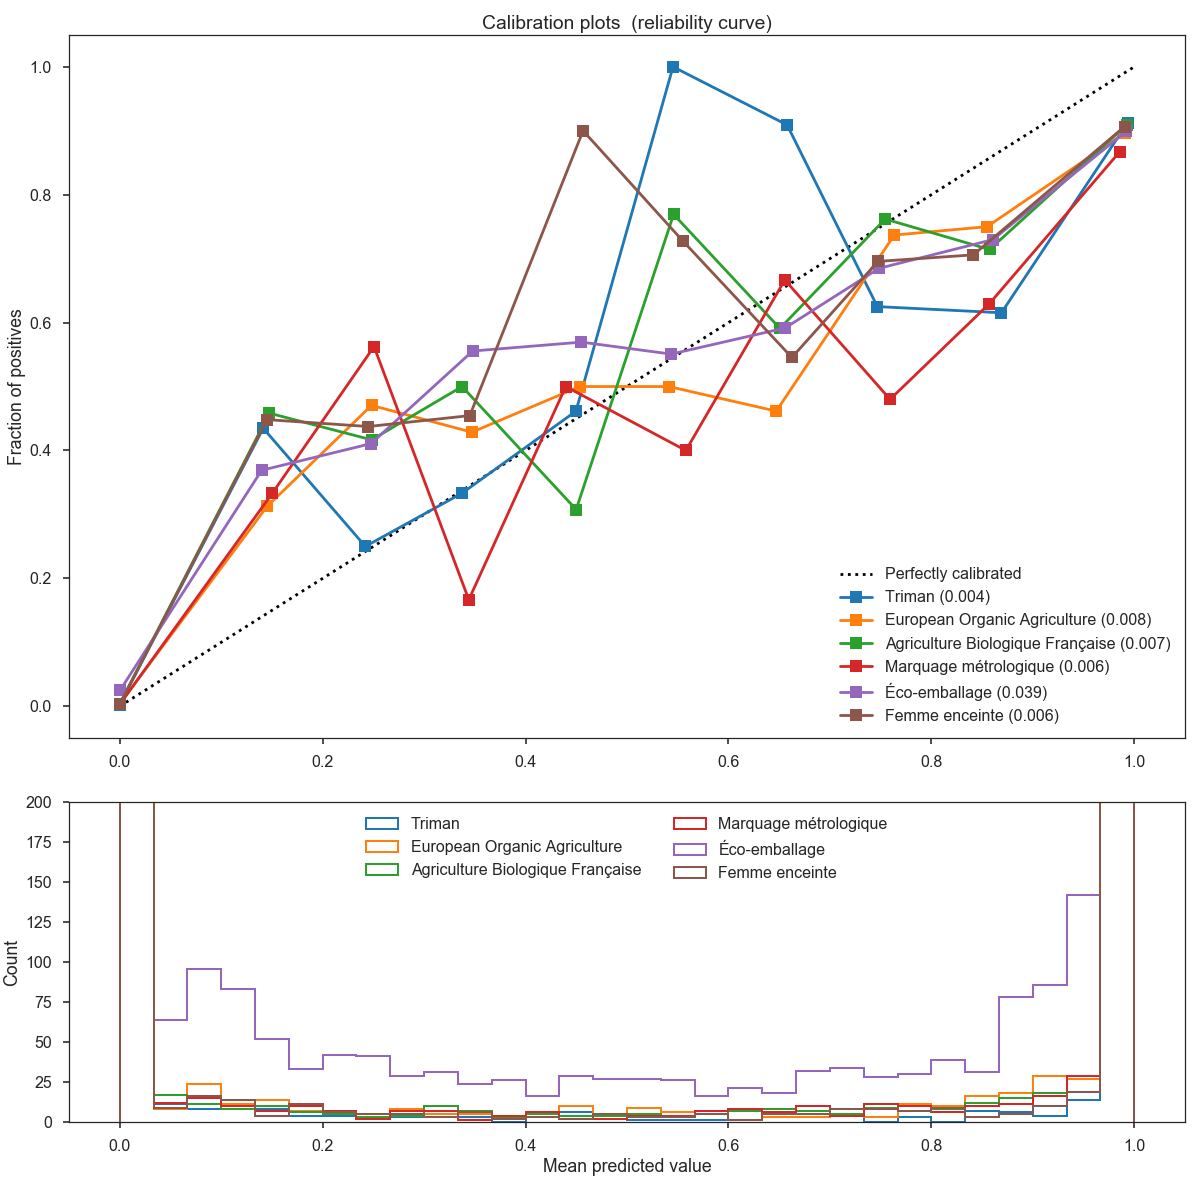
\includegraphics[scale=0.40]{./images/calibration/islabeledby_calibration_curve.png}
\caption{Calibration curve: true precision compared to predicted probabilities/scores.}
\end{figure}

One possible naïve solution would be to build bins of samples around a given score, for instance all scores between 0.40 and 0.50, and estimate the precision of samples in this bin (all prediction whose scores is between 0.4 and 0.5), as the mean precision of that bin on a validation data-set.

\subsection{More advanced calibration techniques}

Major approaches for performing calibration of probabilistic predictions share the same idea: use obtained classification scores as features in an additional classifier (classifier providing scores). We could cite: 
\begin{itemize}
	\item a parametric approach based on Platt’s sigmoid model: basically applying a logistic regression using classification scores as features, and original labels of a validation set as target \cite{Calibration}.
	\item a non-parametric approach based on isotonic regression: the idea is to fit a piecewise-constant non-decreasing function (stair-step shaped).
	\item a 'stacking-style' approach using classification scores as feature, but target are no longer original labels, but the thresholds bipartitioning labels with minimum misclassifications \cite{MultilabelReview}.
\end{itemize}

In our case, we tryed some Platt's and stacking-style calibration techniques, yet given the low label density of our training set, we overfit. However applying isotonic regression provided encouraging results. 

In our case we did not discriminate classes while learning isotonic regression to avoid overfit (micro-average). It was trained on a testing-set and applied on a validation-set. Below charts show results on validation-set before and after isotonic regression. The weighted Brier score slightly dropped from 0.448 to 0.425.

\begin{figure}[H]
\centering
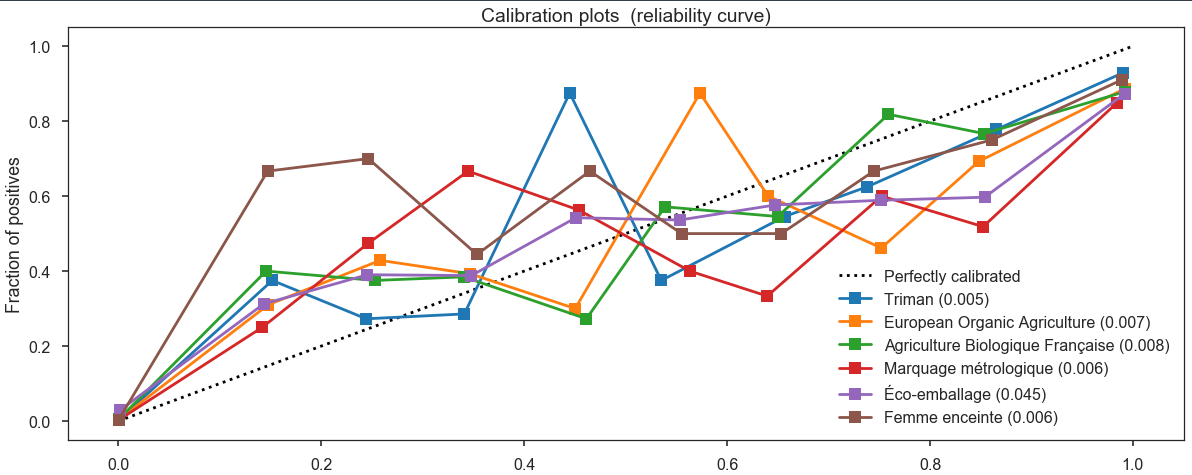
\includegraphics[scale=0.40]{./images/calibration/calibration_val_before.png}
\caption{Calibration curve on validation set BEFORE isotonic regression.}
\end{figure}

\begin{figure}[H]
\centering
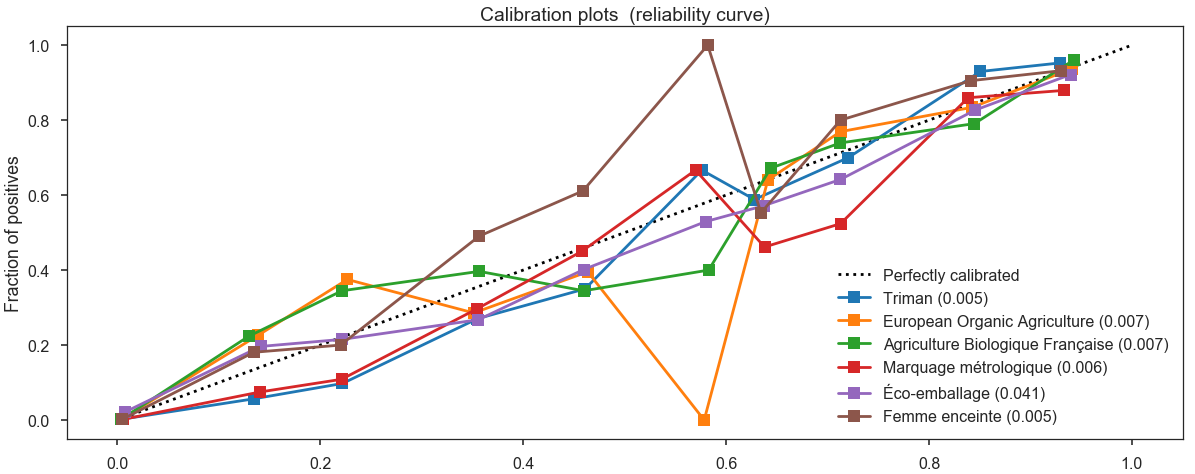
\includegraphics[scale=0.40]{./images/calibration/calibration_val_after.png}
\caption{Calibration curve on validation set AFTER isotonic regression.}
\end{figure}


\subsection{Decision: precision versus recall}

\begin{figure}[H]
\centering
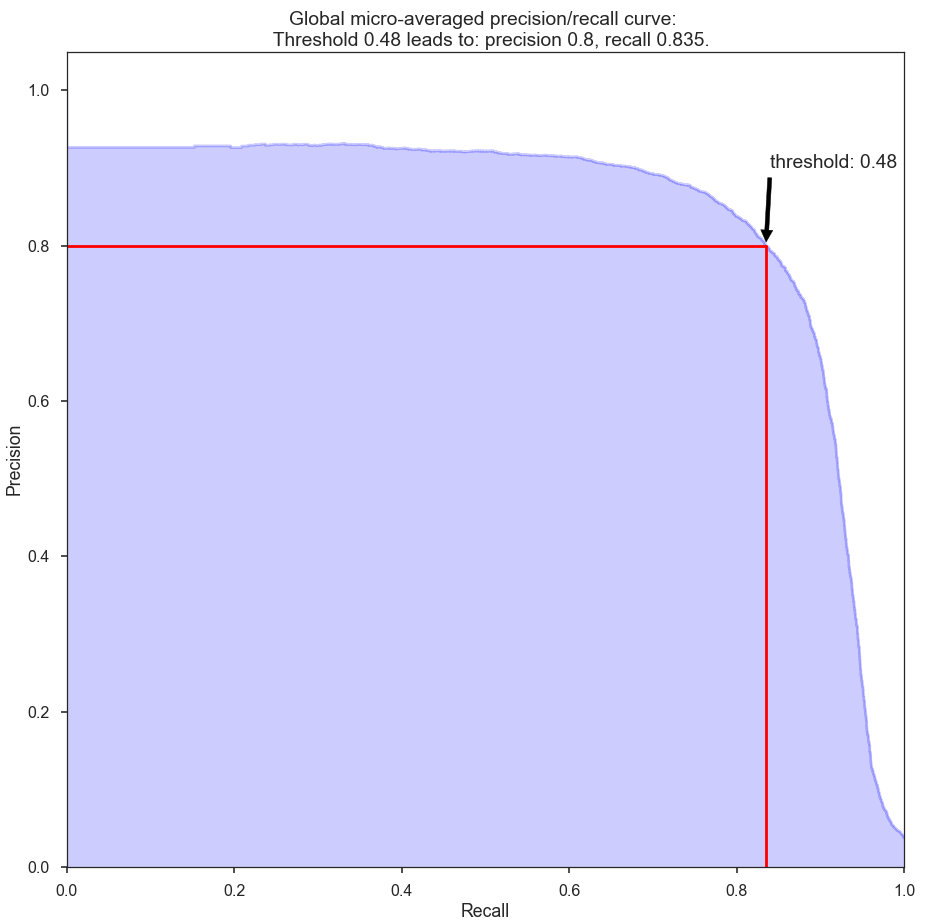
\includegraphics[scale=0.4]{./images/calibration/islabeledby_global_curve.png}
\caption{Global precision/recall curve for attribute 'product labels' (organic, made in France etc).}
\end{figure}

We can observe that if we apply a decision threshold of 0.48 on our prediction scores, we achieve:
\begin{itemize}
	\item a micro-average global precision of 0.80
	\item a micro-average global recall of 0.82
\end{itemize}

Given a decision threshold we will either favor recall or precision, each of them serves a different business objective:
\begin{itemize}
	\item favoring precision ensure that we don't make mistakes when pushing a suggestion to our users, it's a low-risk strategy, but with less impact
	\item favoring recall will ensure that we don't miss any suggestion that we could make on products (big impact), at the risk of being wrong sometimes.
\end{itemize}

The choice is a business choice, depending on what users favor. In our case, after some user interviews, it is clear that we prefer to favor precision. Users are frightened by wrong suggestions. Whereas the absence of suggestion has no negative impact.

\section{Missing labels}

\subsection{Strategies to handle incompletely labeled data}

Our data-quality challenge is quite paradoxical: \textbf{to increase data-quality, we have to rely on the data whose quality we want to improve.}

One issue is then than even if we manage to build a perfect classifier out of this invalid data, when we evaluate it, our precision will be low. Indeed imagine we have 200 products, 100 of them have in reality an 'Organic' label. 40 of them are actually labeled as such in our database (the other 60 being incompletely labeled). If our perfect classifier finds them all, the 100, our classifier precision will be around 40\% instead of 100\% because the test-set on which we will base our estimations will be biaised as well.

To overcome this challenge we adopted the following strategy:

\begin{itemize}
	\item make predictions based on available partially labeled data
	\item enrich our predictions with precision estimation based on each class precision given prediction score (see calibration part)
	\item bulk validate predictions which are not equal to products current attributes, based on:
	\begin{itemize}
		\item either textual search: our prediction are indexed in elasticsearch with product information allowing us to easily look for products whose description fields contain 'gluten'
		\item either categorical search: we know that all alcohols should have a 'pregnant warning pictogram'
		\item either by filtering predictions with the highest precision estimation
	\end{itemize}
	\item validated attributes predictions are stored in a database and override product attributes in classification workflow
\end{itemize}

In the following graphs, you can see that after a initial prediction of flavors attributes, we could detect with high degree a confidence some flavors attributes that were not labeled. After manually validating them, they were incorporated in the learning data-set and increased the training-support for each class. This improved data-quality led to a raise in flavors scores.

\begin{figure}[H]
\centering
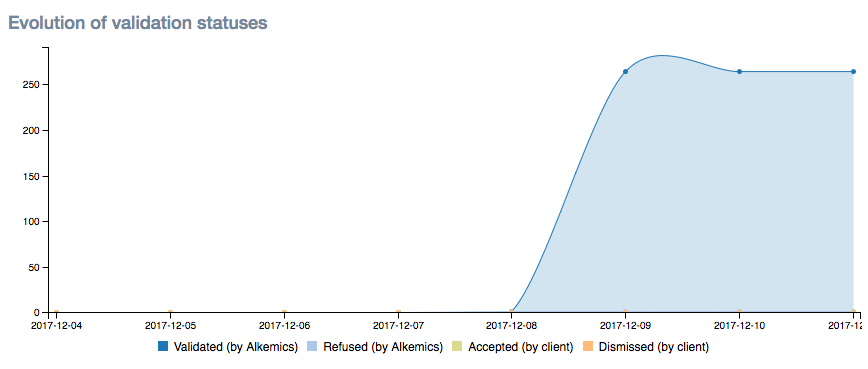
\includegraphics[scale=0.5]{./images/incompletely-labeled/validation-flavors.png}
\caption{Validated flavors predictions. On 2017-12-09, we validated about 250 predictions based on textual search.}
\end{figure}


\begin{figure}[H]
\centering
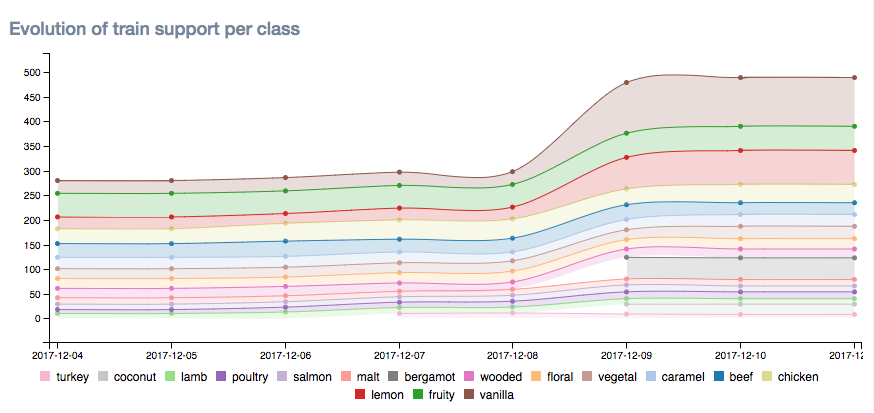
\includegraphics[scale=0.5]{./images/incompletely-labeled/train-support-flavors.png}
\caption{Train support for flavors classes increased as a consequence.}
\end{figure}


\begin{figure}[H]
\centering
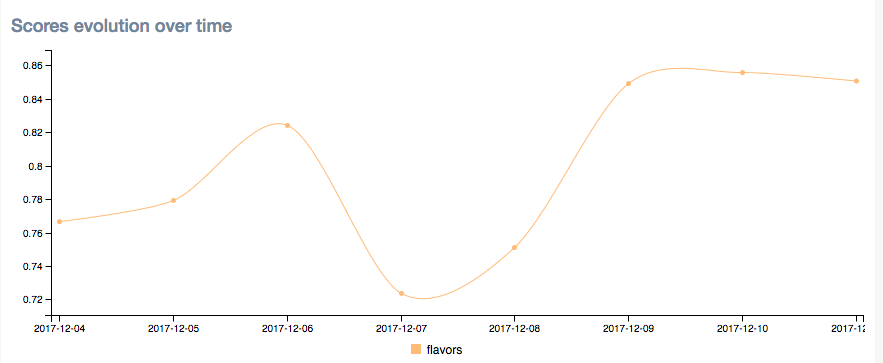
\includegraphics[scale=0.5]{./images/incompletely-labeled/scores-flavors.png}
\caption{Flavors scores are very volatile at the begining because of an insufficient number of training samples. After the validation on 2017-12-08, scores increased and score volatility decreased.}
\end{figure}


This process helps us increase the label density on some classes, which led to increased score.

When we use our predictions with best precision estimation to validate quickly, our process can be seen as a virtuous circle:
\begin{figure}[H]
\centering
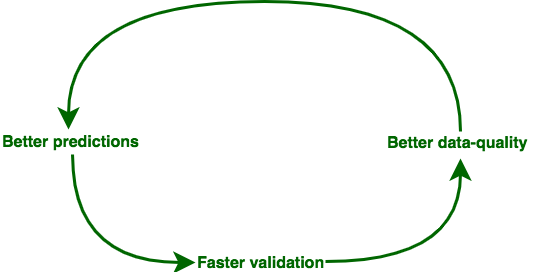
\includegraphics[scale=0.6]{./images/incompletely-labeled/virtuous-circle.png}
\caption{Virtuous validation workflow.}
\end{figure}

Inherently, when training a classifier to detect cases where our data is invalid on some samples, we generally put a stronger focus on precision rather than recall. Indeed:
\begin{itemize}
	\item in multilabel case, our invalid data is in nearly all cases missing values: which will lead to negatives instead of positives in our dataset.
	\item in case we predict a sample as positive for a given class, unfortunatly we will count it as a false positive instead of a true positive.
	\item thus it will impact recall, not precision.
\end{itemize}

\subsection{Iterative approach to bootstrap new classes}

It is sometimes necessary to adopt a pro-active approach on some classes with low scores or very low number of occurences. 
For instance, when we split a 'kind' (category) in multiple more detailed kinds.
After some iterations, there might be enough occurences to ensure sufficient scores.

\section{Evaluate results}

Are we satisfied of our performances, could we do better or not given the task difficulty? Even though we will detail in next section the fields we want to investigate further to improve our models, these are difficult questions for which our answers cannot be definitive.

\subsection{Assess task difficulty}
Task difficulty can be assessed differently for each predicted field. It is dependent on multiple factors:
\begin{itemize}
	\item output size
	\begin{itemize}
		\item multiclass vs multilabel
		\item number of distinct classes
	\end{itemize}
	\item number of training samples
	\begin{itemize}
		\item dataset size
		\item classes and label densities: it will be difficult to predict labels that nearly never occur
	\end{itemize}
	\item is the information present in some form in features
	\begin{itemize}
		\item flavors are usually nearly textually present in features (textual composition, or description)
		\item in contrast to kind (category) which are not necessarly textually present
	\end{itemize}
\end{itemize}

\begin{tabularx}{\textwidth}{|l|r|X|X|X|X|X|r|}
\toprule
field & type &  label\ count & label\ cardinality &  label\ density &  label\ diversity &  nb\ classes &  nb\ samples \\
\midrule
hazard			      &          multilabel &    2243     &     0.0408 &         0.0082 &             1090 &           5 &       54990\\
flavors               &          multilabel &    355      &     0.0065 &         0.0006 &              253 &          11 &       54990 \\
kind                  &          multiclass &    43335    &     1.0000 &         0.0057 &              175 &         175 &       43335 \\
ingredients			  &          multilabel &    54259    &     0.9867 &         0.0111 &            16810 &          89 &       54990 \\
labels 		          &          multilabel &    22803    &     0.4147 &         0.0078 &             7078 &          53 &       54990 \\
\bottomrule
\end{tabularx}


\subsection{Assess how well our model perform}

Here are the scores obtained applying on our classes scores a global threshold maximizing f1-score:

\textbf{Micro average scores}
\begin{tabular}{lrrr}
\toprule
{} &  f1\_score &  precision &   recall \\
fieldmetadata\_name    &           &            &          \\
\midrule
hazardpictograms      &   0.808 &    0.833 &  0.784 \\
hasnotableingredients &   0.745 &    0.755 &  0.735 \\
kind                  &   0.882 &    0.882 &  0.882 \\
flavors               &   0.403 &    0.552 &  0.318 \\
islabeledby           &   0.794 &    0.803 &  0.785 \\
\bottomrule
\end{tabular}

\textbf{Macro average scores}
\begin{tabular}{lrrr}
\toprule
{} &  f1\_score &  precision &   recall \\
fieldmetadata\_name    &           &            &          \\
\midrule
hazardpictograms      &   0.788 &    0.834 &  0.751 \\
hasnotableingredients &   0.544 &    0.523 &  0.605 \\
kind                  &   0.787 &    0.785 &  0.805 \\
flavors               &   0.348 &    0.479 &  0.294 \\
islabeledby           &   0.626 &    0.613 &  0.690 \\
\bottomrule
\end{tabular}

As a reminder:
\begin{itemize}
 	\item in our case given the disparity of size classes we will generally consider micro rather than macro score.
 	\item macro scores are very impacted by the fact that many classes have very few occurences and perform badly
 	\item it is difficult to evaluate how much the errors are due to a wrongly qualified classifier, versus due to uncompletely labeled data. Indeed for a given decision threshold recall scores might be underestimated
\end{itemize}


\subsection{How much better can we do}

To answer this question, one must first evaluate what is current data-quality. We can certainly do better but have no specific metrics to estimate it. Still we have reasons to be optimistic, the data we are relying on is quickly growing, which will naturally improve our models (our models local performances are strongly correlated to classes support), and we already managed to bootstrap many fields and classes. Plus the following section will cover our thoughts to improve our current workflow.


\section{To investigate further}

This section cover some topics we have not had time to cover for now, and that we think could help us deliver better results.

\subsection{Dive into kind tree-structure}
One of the attributes we predict has a tree structure: the 'kind', or product category. 

\begin{figure}[H]
\centering
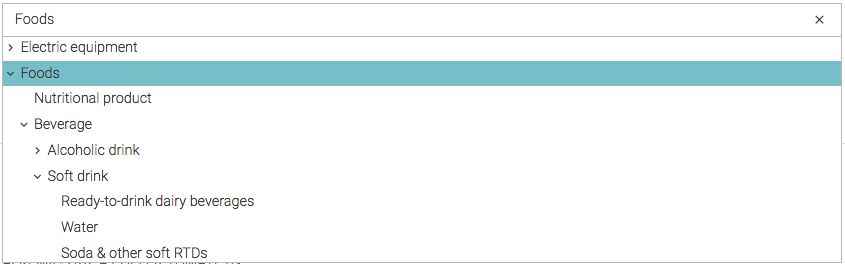
\includegraphics[scale=0.5]{./images/to-investigate/tree-structure.png}
\caption{Kind tree structure: Food contains Beverage, that contains Soft-dring, that contains Water, Soda etc..}
\end{figure}

We could take advantage of the information contained in the tree structure to improve classification. 

One possible strategy could be to create a kind similarity function, returning a scalar based on proximity in tree structure:
\begin{itemize}
	\item 'water' is very close to 'soft drink' because it is its direct child
	\item 'water' and 'bread' are very different because the shortest path between them is 4 edges.
\end{itemize}

This similarity function could be used as a coefficient in the cost function: 
\begin{itemize}
	\item if we predict 'soft drink' instead of 'water', the cost would be lowered because the error is minor
	\item if we predict 'bread' instead of 'water', the cost would be raised because the prediction is completely wrong
\end{itemize}

\subsection{Use images as input}

For now, use of google vision API to product text: labels, reading. 

This extracted features could be used in our workflow, but we might also change our model to some neural networks embedding different types of objects. Facebook recently released a library to embbed different types of objects \cite[starspace]{wu2017starspace}.


\subsection{Part of Speech Tagging strategies to predict some fields}
Some attributes are usually present in description (brand, packaging etc). These element might be detectable through part of speech tagging methods.

\subsection{Tuning strategies}

For now tuning was done quite intuitively, but given the very large size of parameters space we have room for improvement.

\subsection{Higher order multilabel strategies}
Possible strategies include:
\begin{itemize}
	\item add layer to Fasttext neural network
	\item add independent layer, at the end: calibration (that will find correlation between classes)
\end{itemize}

Yet, these strategies are possible only with datasets with sufficient samples, otherwise we will overfit.

\subsection{Cross validation for sets with low label density}

Our monitoring dashboard allow us to see scoring metrics evolution. These scoring metrics are computed at training stage on a testing set. We observed that some metrics were volatile because when not much support samples were available for a given field.

\subsection{More workflow tests}
We encountered some inconsistencies that appeared to be due to errors in the workflow. We are currently adding some more tests to avoid this kind of error in the future.

\subsection{Estimate data-quality on predicted attributes on sample}
One (time-consuming but) interesting experiment would be to manually assess data-quality on a sufficiently large and representative dataset. This would help us estimate our classifier real performances.

